%!TEX root = main.tex
\section{A-Graphs}
\seclabel{quad}
\seclabel{quadrangulations}

In this section, we study a special class of graphs that are closely
related to quadrangulations in which every edge crosses $Y$. (See \figref{a-graph} for an example.)

\begin{definition}\deflabel{a-graph}
	An \emph{A-graph}, $G$, is a \Fary\ embedding of a graph with $n\ge 3$ vertices that has the following properties:
	\begin{compactenum}
		\item Every edge of $G$ intersects $Y$ in exactly one point, possibly an endpoint.
		\item Every face of $G$, including the outer face, is a quadrilateral or a triangle.
		\item Every quadrilateral face of $G$ is non-convex.
		\item Every triangular face contains one vertex in each of $Y$, $L$,
		and $R$.  
		\item Every vertex $v$ on $Y$ is incident to precisely
		two triangular faces, one ``above $v$'' whose interior contains the open line segment with endpoints $v$ and $v+(0,\epsilon)$ for some $\epsilon>0$ and one ``below $v$'' whose interior contains the open line segment with endpoints $v$ and $v-(0,\epsilon)$ for some $\epsilon >0$.
	\end{compactenum}
\end{definition}

\begin{wrapfigure}[11]{r}{.3\textwidth}
		\vspace{-1mm}
		\centering
		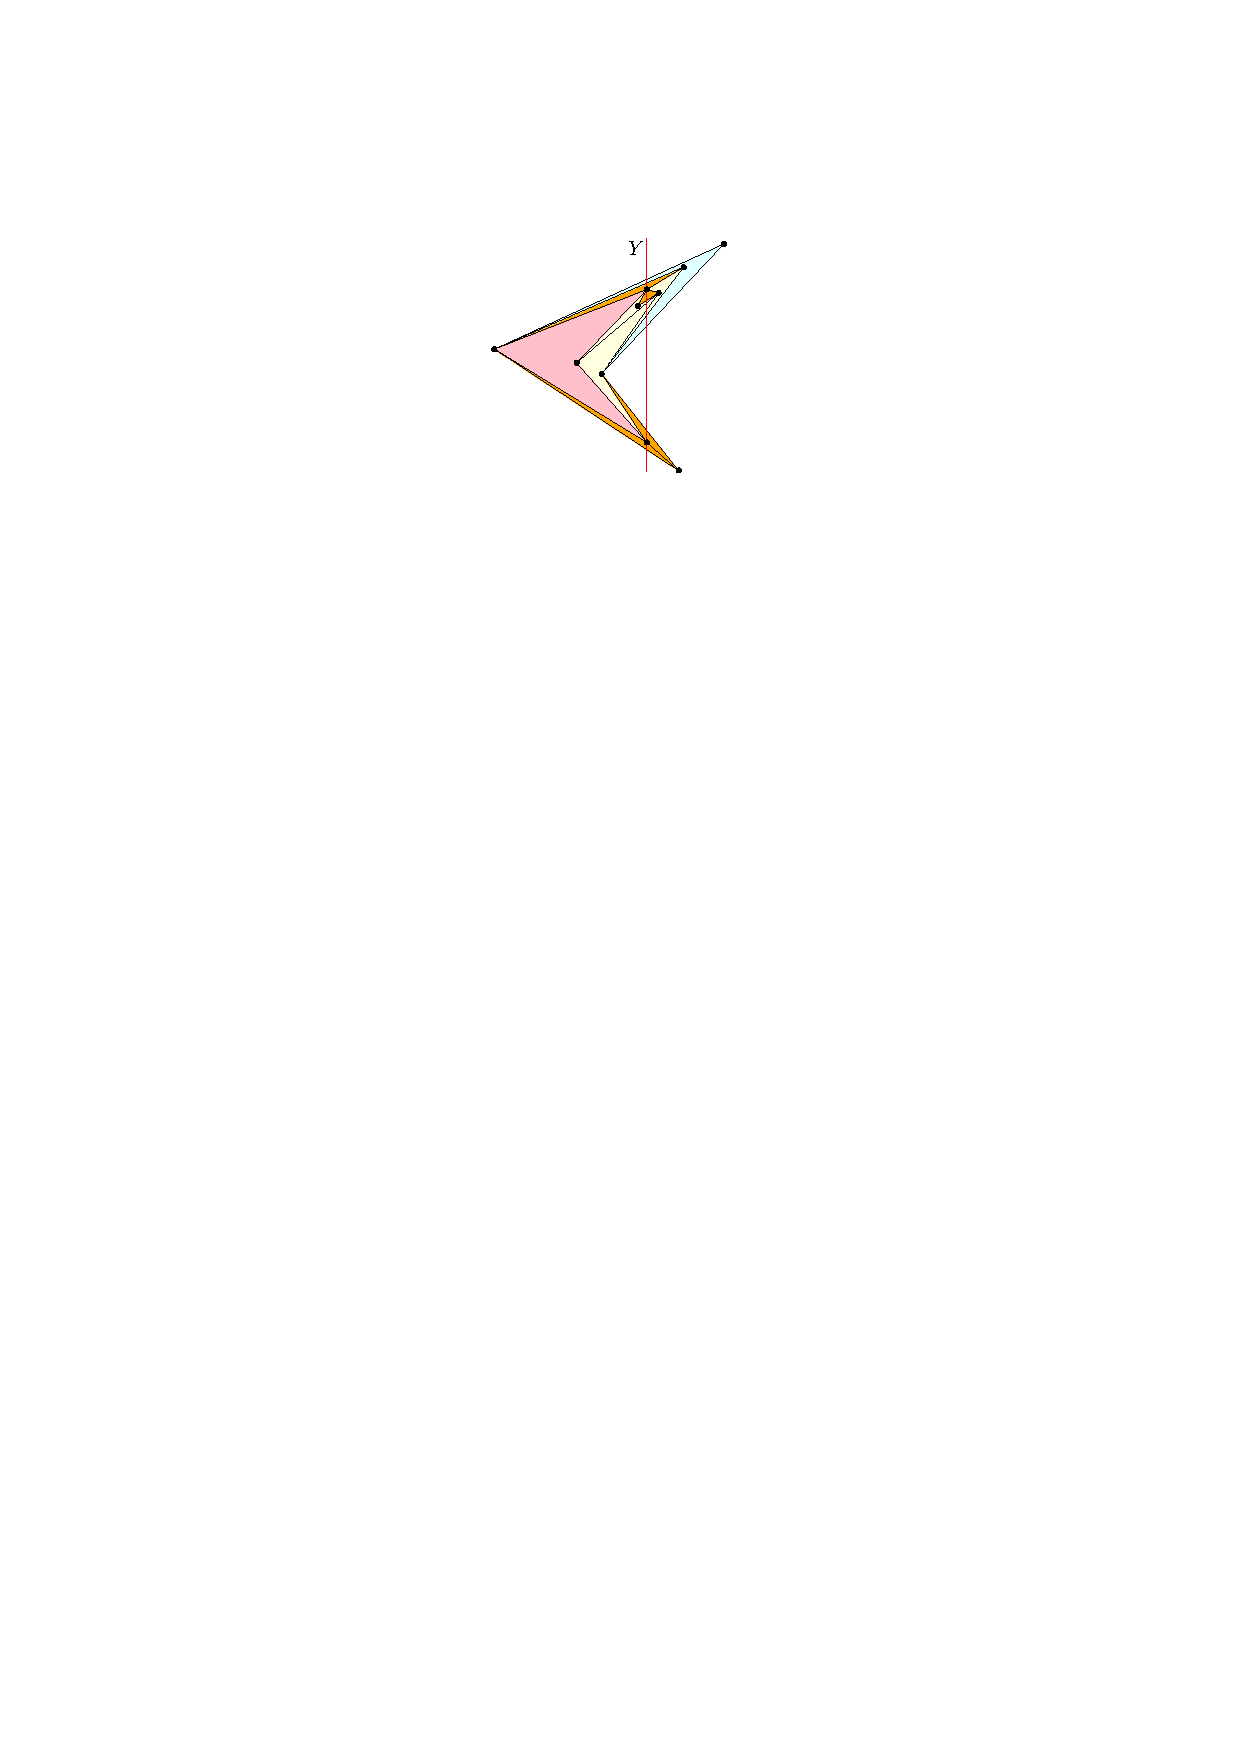
\includegraphics[scale = 0.95]{figs/a-graph-new}
		\caption{An A-graph with 2 vertices in $Y$.}
		\figlabel{a-graph}
	\end{wrapfigure}
	
In the special case where $G$ has no vertices in $Y$, the graph $G$ is a quadrangulation in which every edge crosses $Y$. Further, Property~5 applies even if $v$ is on the outer face of $G$ (in which case it implies that the outer face of $G$ must be a triangle).
Some additional properties of $G$ follow from \defref{a-graph}:
\begin{compactenum}\setcounter{enumi}{5}
	\item $G$ is connected.
	\item Every vertex of $G$ has degree at least 2.   
	\item If $n\ge 4$, then every vertex in $Y$ has degree at least 3. 
\end{compactenum}
Property~6 follows directly from Property~2.
Property~7 follows from the fact that every vertex is incident to at
least one face and every face is a simple cycle.
Property~8 follows from the fact that every vertex on $Y$ is incident
to at least two triangular faces, which involve at least 4 vertices, unless $n=3$.

%We will show that every A-graph $G$ has a \Fary\ embedding with prescribed
%intersections with $Y$ and a prescribed outer face.  Since the outer
%face of an A-graph can be a triangle or a quadrilateral, in the following
%theorem, $\Delta$ is a triangle or quadrilateral defined as follows:
%\begin{enumerate}
%   \item If $(0,y_1)$ is a vertex of $G$, then $\Delta$ is a triangle
%   with one vertex at $(0,y_1)$ and the opposite edge edge crossing $Y$ at $y_m$.
%
%   \item If $(0,y_m)$ is a vertex of $G$, then $\Delta$ is a triangle
%   with one vertex at $(0,y_m)$ and the opposite edge crossing $Y$ at $y_1$.
%
%   \item Otherwise,
%      $\Delta$ is a quadrilateral whose edges cross $Y$ at $y_1$, $y_a$,
%      $y_b$, and $y_m$, where $e_1$, $e_a$, $e_b$, and $e_m$ are the four edges on the outer face of $G$
%\end{enumerate}

We will show that every A-graph $G$ has a \Fary\ embedding with prescribed intersections with $Y$ and a prescribed outer face, as in the following theorem. 

\begin{thm}\thmlabel{a-graph}
	Let
	\begin{compactenum}
		\item $G$ be an A-graph;
		\item $e_1,\ldots,e_m$ be the sequence of edges in $G$,
		in the order they are intersected by $Y$;
		\item $y_1\le\cdots\le y_m$ be any sequence of numbers where, for
		each $i\in\{1,\ldots,m-1\}$, $y_i=y_{i+1}$ if and only if $e_i$
		and $e_{i+1}$ have a common endpoint in $Y$;
		\item $\Delta$ be a triangle or quadrilateral, where:
		\begin{compactenum}
			\item If $(0,y_1)$ is a vertex of $G$, then $\Delta$ is a triangle
			with a vertex at $(0,y_1)$ and the opposite edge crossing $Y$ at $y_m$.
			
			\item If $(0,y_m)$ is a vertex of $G$, then $\Delta$ is a triangle
			with a vertex at $(0,y_m)$ and the opposite edge crossing $Y$ at $y_1$.
			
			\item Otherwise, $\Delta$ is a quadrilateral whose edges cross $Y$ at $y_1$, $y_a$,
			$y_b$, and $y_m$, where $e_1$, $e_a$, $e_b$, and $e_m$ are the four edges on the outer face of $G$.
		\end{compactenum}
	\end{compactenum}
	Then $G$ has a
	\Fary\ embedding in which the outer face is $\Delta$
	and, for each $i\in\{1,\ldots,m\}$, the intersection between $e_i$ and $Y$
	is the single point $(0,y_i)$.
\end{thm}

%%%%% copia da qui %%%%%%
The rest of this section is devoted to prove \thmref{a-graph}. We make some simplifying assumptions. First, we assume w.l.o.g.\ up to a uniform scaling that $\Delta$ and all the vertices of $G$ are contained in $[-1,1]^2$. Second, we assume w.l.o.g.\ up to a reflection  with respect to $Y$ that, if the outer face of $G$ is delimited by a quadrilateral, then the vertex incident to both $e_1$ and $e_m$ is in $L$, as in \figref{a-graph}. In such a case we also assume that the vertex of $\Delta$ incident to both $e_1$ and $e_m$ is in $L$; this is also not a loss of generality, as if the vertex of $\Delta$ incident to both $e_1$ and $e_m$ is in $R$, then $\Delta$ can be reflected with respect to $Y$, obtaining a quadrilateral $\Delta'$ whose vertex incident to both $e_1$ and $e_m$ is in $L$, then a \Fary\ embedding of $G$ can be constructed in which the outer face is $\Delta'$, and finally the \Fary\ embedding can be reflected with respect to $Y$, thus obtaining a \Fary\ embedding of $G$ in which the outer face is $\Delta$. 

If $m=3$ or $m=4$, then $G$ is a 3- or a 4-cycle, respectively, hence it suffices to embed it as $\Delta$. Therefore we assume, from now on, that $m\ge 5$.  
%%%%% copia fino a qui %%%%%%

	\begin{wrapfigure}[10]{r}{.32\textwidth}
		\vspace{-1mm}
		\centering
		\includegraphics[scale = 0.95]{figs/ab}
		\caption{The ordering of the edges incident to a vertex $v$ on $Y$.}
		\figlabel{ab}
	\end{wrapfigure}
Before continuing, we pause to fully specify the ordering
$e_1,\ldots,e_m$. This ordering is unambiguous except where
some vertex $v\in Y$ is incident to several edges
$e_{i},\ldots,e_{i+d}$, where $d\ge 2$ by Property~8 of A-graphs. Refer to \figref{ab}.  In this case we partition $v$'s neighbors into two
sets $\alpha_1,\ldots,\alpha_k\in L$ and $\beta_1,\ldots,\beta_\ell\in
R$, where $\alpha_1,\ldots,\alpha_k$ are ordered clockwise around $v$
and $\beta_1,\ldots,\beta_\ell$ are ordered counterclockwise.  We then use
the convention that $e_i,\ldots,e_{i+k-1}=v\alpha_1,\ldots,v\alpha_k$
and $e_{i+k},\ldots,e_{i+d}=v\beta_1,\ldots,v\beta_\ell$.

We will describe the desired \Fary\ embedding by assigning a slope
$s_i$ to each edge $e_i\in E(G)$.  
Since there can be no vertical edges, each slope $s_i$ is well-defined.
We have $m=|E(G)|$ slope variables, $s_1,\ldots,s_m$.  Since every edge
$e_i$ contains the point $(0,y_i)$, the slope $s_i$
fixes the line through $e_i$.  Since every vertex $v$ not on $Y$ is
incident to at least two edges that contain distinct points on $Y$,
the location of $v$ is fixed.  (The location of each vertex on $Y$
is fixed by definition.)

A necessary condition for the slopes to determine a F\'ary embedding of $G$ is that the supporting lines of edges 
with a common vertex should be concurrent. Let $v$ be a vertex 
not on $Y$, and let $e_i, e_j, e_k$ be three edges incident to $v$.
The fact that the supporting lines of $e_i$, $e_j$, and $e_k$
meet at a common point (the location of $v$) is expressed by the following
\emph{concurrency constraint} in terms of the slopes $s_i,s_j,s_k$:
\begin{equation}\eqlabel{slope0} 
\left|
\begin{matrix}
1&1&1\\
s_i&s_j&s_k\\
y_i&y_j&y_k
\end{matrix}
\right|=
({y_j-y_k}) s_i + ({y_k-y_i}) s_j 
+ ({y_i-y_j})s_k  = 0
\end{equation}
Since $y_1,\ldots,y_m$ are given, this is a linear equation
in $s_1,\ldots,s_m$.
Writing this equation for all triplets of edges incident to a common
vertex $v$ will include many redundant equations. Indeed, it suffices to take $d_v-2$ equations: We choose two fixed
incident edges $e_i$ and $e_j$ and run $e_k$ through the remaining
$d_v-2$ edges, specifying that $e_k$ should go through the common vertex
of $e_i$ and $e_j$.
%We call the resulting collection of $\sum_{v\in V(G)\setminus Y} d_v-2$ equations the \emph{concurrency constraints}.

Whenever convenient, we will use edges of $G$
as indices so that, if $e=e_i$ is an edge of $G$, then $s_e=s_i$
and $y_e=y_i$.  Further, if $e$ is a line segment that
intersects $Y$ in a point, we will use $y_e$ to denote the $y$-coordinate
of the intersection of $e$ and $Y$ and $s_e$ to denote the slope of
$e$'s supporting line.

%It will be important to have as many equations as variables;
%thus, 

We now introduce additional equations for the edges that emanate from a
vertex on $Y$.
Suppose that a vertex $v\in Y$ is incident to edges $a_1,\ldots,a_k\in L\cup Y$ 
and $b_1,\ldots,b_\ell\in Y\cup R$, ordered from bottom to top as in \figref{ab}.
From Property~4 of A-graphs we have $k,\ell\ge1$ and, from Property~8, we have $k+\ell\ge 3$.
Let us first look at the slopes on the right side.
We want these slopes to be increasing:
$s_{b_1} < s_{b_2} < \dots  <s_{b_\ell}$. We stipulate a stronger
condition:
We require that the slopes
$s_{b_2}, \dots, s_{b_{\ell-1}}$ partition the interval
$[s_{b_1},s_{b_\ell}]$ in fixed proportions. In other words:
\begin{equation}
\label{eq:proportion}
s_{b_i} = s_{b_1} + \lambda_i(s_{b_{\ell}}-s_{b_1}),
\end{equation}
for some fixed sequence $0<\lambda_2<\cdots<\lambda_{\ell-1}<1$.

For example, we might set $\lambda_i := (i-1)/(l-1)$.
This gives $\ell-2$ equations, for $\ell\ge 2$. Similarly, we get
$k-2$ equations for the slopes
$s_{a_1}, \dots, s_{a_{k}}$ of the edges on the left side, for $k\ge 2$.
In addition, for $k\ge 2$ and $\ell\ge 2$, we require that the \emph{range} of
slopes
on the two sides are in a fixed proportion:
\begin{equation}
\label{eq:proportion2}
s_{a_1}-s_{a_{k}} = \mu (s_{b_{\ell}}-s_{b_1}),
\end{equation}
for some fixed value $\mu>0$.

We call the equations
\thetag{\ref{eq:proportion}--\ref{eq:proportion2}} the
\emph{proportionality constraints}.
There are $(k+\ell)-3$ such equations for the $k+\ell$ slopes, hence we have three degrees of freedom for the slopes out of a vertex.
%\figref{proportional} illustrates these  degrees of freedom:
Namely, we can shear the edges on the right side vertically, adding the same constant to all
slopes. We can independently shear all edges on the left side.
In addition, we can vertically scale {all} lines jointly (both to
the left and to the right), multiplying all slopes by the same constant factor.
If this factor is negative, we would reverse the order of the
slopes, simultaneously on the left and on the right. We will later see how to prevent this. We can already observe that two slopes on one side determine all remaining slopes on that side. Moreover, the range of slopes on the other side ($s_{a_1}-s_{a_{k}}$ or $s_{b_{\ell}}-s_{b_1}$) is also determined.
%
The notations $\lambda_i$ and $\mu$ are here used in a local sense;
for a different vertex $v$, we may choose different constants.
%\begin{figure}
%	\centering{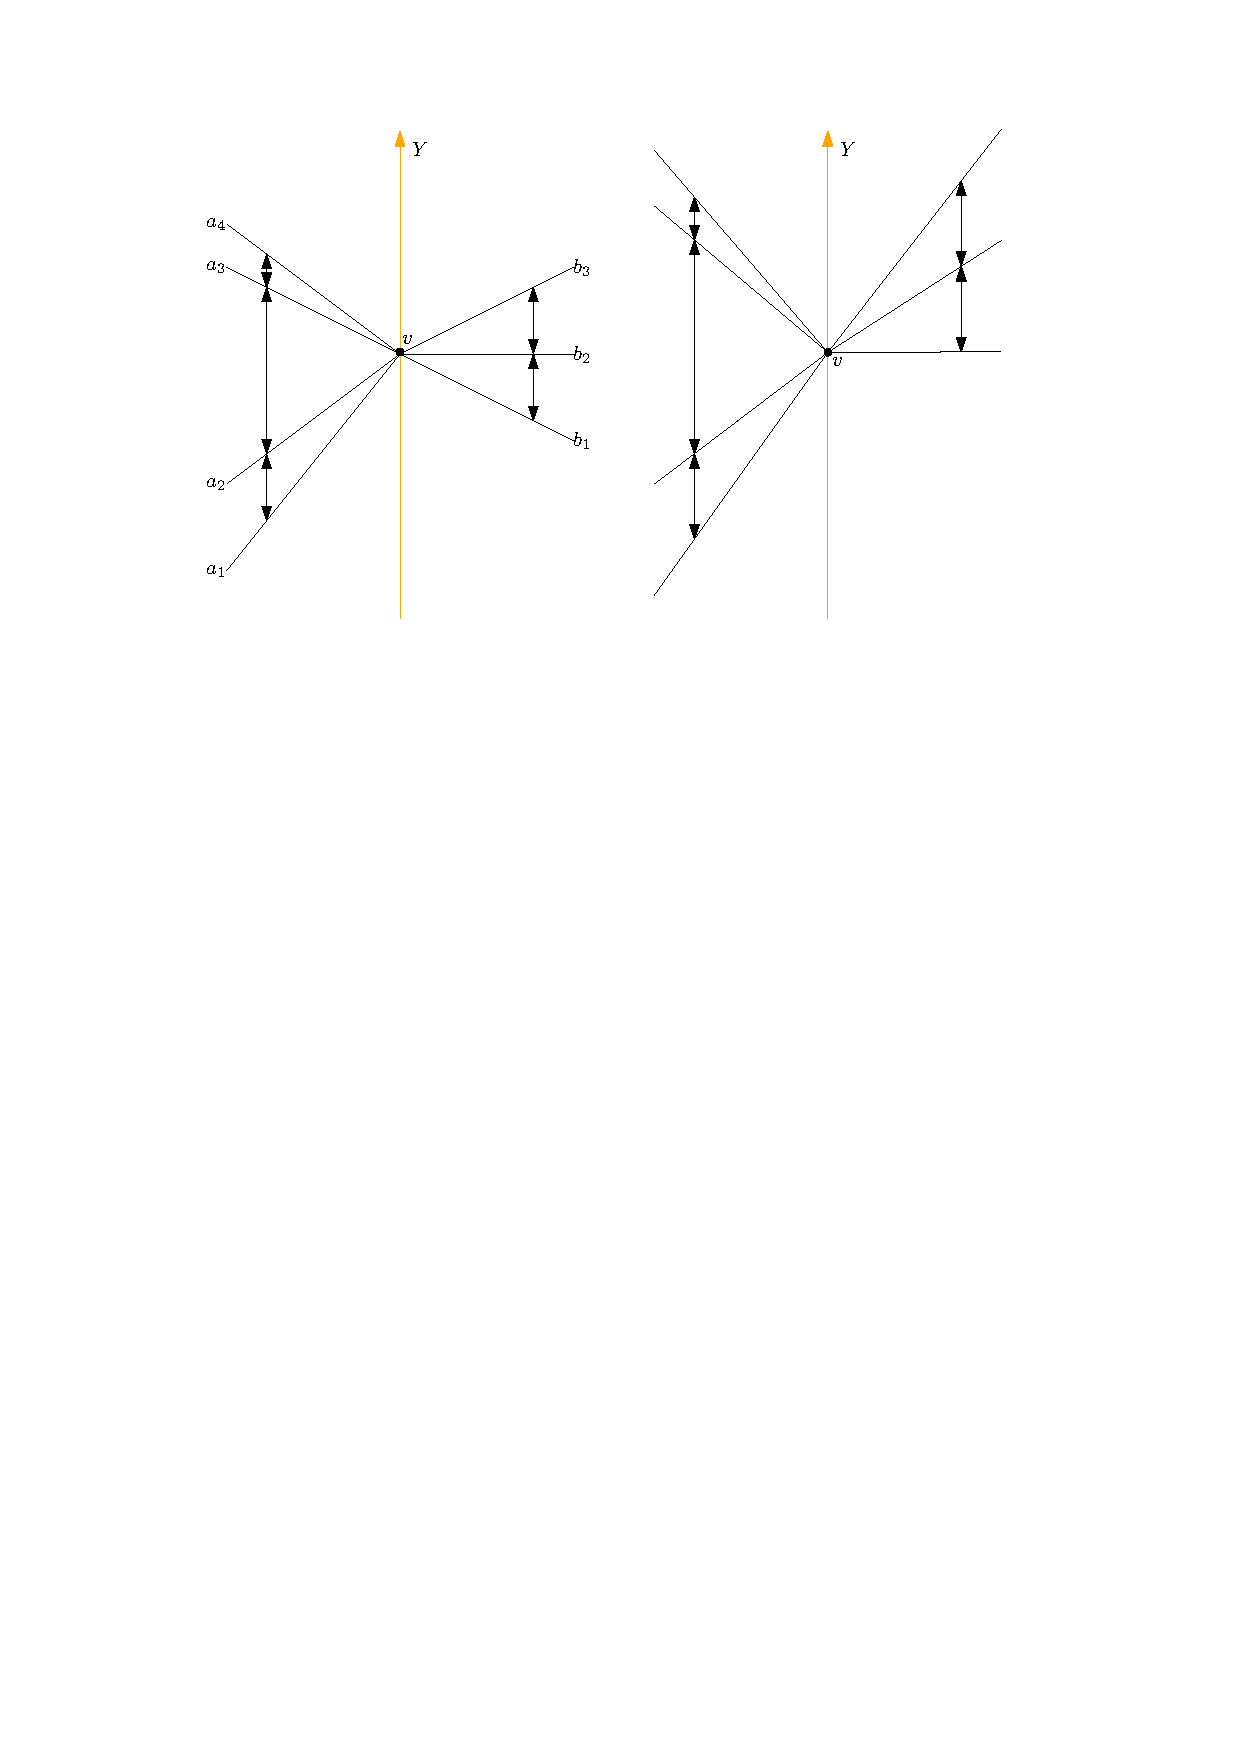
\includegraphics{figs/proportional}}
%	\caption{The degrees of freedom provided by the proportionality constraints}
%	\figlabel{proportional}
%\end{figure}
We have the following.
\begin{lem} \label{le:number-of-equations}
The total number of equations \thetag{\ref{eq:slope0}},~\thetag{\ref{eq:proportion}}, and~\thetag{\ref{eq:proportion2}} is $m-4$.
\end{lem} 
\begin{proof}
Let $n=|V|$ and let $n_0$ be the number
of vertices on $Y$. Assume that $G$ has $f_3$ triangular and $f_4$
quadrangular faces.

Two triangles for every vertex on $Y$ (Property 5 of A-graphs):
\begin{equation}
\label{eq:f3}
f_3 = 2n_0
\end{equation}
Euler's formula:
\begin{equation}
\label{eq:Euler}
n + f_3+f_4 = m+2
\end{equation}
Double-counting of edge-face incidences leads to the relation
\begin{equation}
\label{eq:edge-face}
3f_3+4f_4=2m.
\end{equation}
We have $d_v-3$ equations for each of the $n_0$ vertices $v$ on $Y$. For each of the 
$n-n_0$ vertices $v$ not on $Y$, 
we have $d_v-2$ equations.
The total number of equations is therefore
\begin{align*}
% \label{eq:number-equations2}
P &= 
\sum_{v\in V(G)\cap Y}^n(d_v-3)+
\sum_{v\in V(G)\cap(L\cup R)}^n(d_v-2)
=
\sum_{v\in V}^n(d_v-2)-n_0
=
2m-2n-n_0.
\end{align*}
Using \thetag{\ref{eq:f3}--\ref{eq:edge-face}}, this can be
simplified to
\begin{align*}
P&=
2m-2n-n_0\\
&= 2m -2n -2f_3-2f_4 +2f_3+2f_4-n_0\\
&= 2m -2(n +f_3+f_4) +\tfrac12(4f_3+4f_4-f_3)\\
&= 2m -2(m+2) +m = m-4.
\end{align*}
This concludes the proof of the lemma.
\end{proof}

To achieve the desired number, $m$, of equations, we add
four \emph{boundary equations}.  If the outer face is a quadrilateral, we set
the slopes $s_1$, $s_a$, $s_b$, and $s_m$ of its edges $e_1$, $e_a$, $e_b$, and $e_m$ to the fixed values of the slopes of the edges of $\Delta$. If the outer face is a triangle $\alpha\beta\gamma$, with $\gamma\in Y$, we set the slopes $s_1$, $s_a$, and $s_m$ of the boundary edges $e_1$, $e_a$, and $e_m$ to the fixed values of the slopes of the edges of $\Delta$ and we pick another (non-boundary) edge $e_b$ incident to $\gamma$ and set its slope $s_b$ to a fixed value; this value is such that $s_b$ is either larger than each of $s_1$, $s_a$, and $s_m$ or smaller than each of $s_1$, $s_a$, and $s_m$, depending on whether the slope of $e_b$ in $G$ is larger than the slope of each of $e_1$, $e_a$, and $e_m$ or smaller than the slope of each of $e_1$, $e_a$, and $e_m$. Observe that no other cases are possible. Together with the proportionality constraints, this effectively pins all the slopes incident to $\gamma$ to fixed values.

Altogether, we have now a system of $m$ linear equations
in the $m$ unknowns $s=(s_1,\ldots,s_m)$, which we can write
compactly as
$A\cdot s = b$, with a square matrix $A$ whose entries come from
\thetag{\ref{eq:slope0}--\ref{eq:proportion2}}.
%are the variables we wish to solve for, and $b$ is a column $m$-vector
%whose entries also come from \eqref{slope}.  
Only four entries of
the right-hand side vector
$b$
are non-zero, due to the four boundary equations.
We will show that $A\cdot s=b$ has a unique
solution and that this solution gives a \Fary\ embedding of $G$.

\subsection{Setting Proportionality Constraints}

%Since our plan is to show how to morph the given embedding of $G$ into the desired embedding, it is important that the given embedding satisfy the appropriate system of equations.  

We now specify how the coefficients in the proportionality constraints
are chosen, so that they are satisfied by the initial embedding.  The statement of \thmref{a-graph} assumes that $G$ is a \Fary\ embedding.  In this embedding, every edge $e$ intersects $Y$
in a single point $(0,y_e')$ and has a slope $s_e'$.  For a particular
vertex $v\in Y$, incident to edges $a_1,\ldots,a_k$ and $b_1,\ldots,b_\ell$
as described above, we use the slopes in the given embedding to set the
coefficients in the proportionality constraints.  In the notation used
in \eqref{proportion}, we set
\[
\lambda_i = (s_{b_i}'-s_{b_1}')/(s_{b_\ell}'-s_{b_1}') 
\]
and in \eqref{proportion2}, we set
\[
\mu = (s_{a_1}'-s_{a_k}')/(s_{b_\ell}'-s_{b_1}') \enspace .
\]
This ensures that the slopes $s_{e_1}',\ldots,s_{e_m}'$ satisfy the
proportionality constraints.


\subsection{Ordering constraints}

We define a relation $\prec$ on the edges of $G$, where $e_1 \prec e_2$ if and only if
\begin{enumerate}
	\item $y_{e_1} < y_{e_2}$ and $e_1$ and $e_2$ have a common endpoint $v\in L$; or
	\item $y_{e_1} > y_{e_2}$ and $e_1$ and $e_2$ have a common endpoint $v\in R$.
\end{enumerate}
We say that a vector $s=(s_1,\ldots,s_m)$ \emph{satisfies the ordering
	constraints} if $s_{e_1} < s_{e_2}$ for every pair $e_1,e_2\in E(G)$
such that $e_1\prec e_2$. This definition captures the condition that vertices of $G$ in $L$ (respectively, $R$) should be embedded so that they remain in $L$ (respectively, $R$), as in the following. 

\begin{obs}\obslabel{left-right}
If a solution $s$ to $A\cdot s=b$ satisfies the ordering constraints, then every vertex that is in $L$ (in $R$) in $G$ is also in $L$ (respectively in $R$) in the embedding corresponding to $s$. 
\end{obs}

\begin{proof}	  
Consider any vertex $v$ that is in $L$ in $G$ and that is incident to (at least) two edges $e_1$ and $e_2$. Assume w.l.o.g.\ that $y_{e_1} < y_{e_2}$, and hence that $e_1 \prec e_2$. Since $s$ satisfies the ordering constraints we have $s_{e_1} < s_{e_2}$, hence the lines with slopes $s_{e_1}$ and $s_{e_2}$ through $(0,y_{e_1})$ and $(0,y_{e_2})$, respectively, meet in $L$. The argument for the vertices in $R$ is analogous. 
\end{proof}	  

Note that $\prec$ is acyclic since $G$ is an A-graph and therefore the slopes $s_{e_1}',\ldots,s_{e_m}'$ of edges
in $G$ satisfy the ordering constraints.  This would not be possible if $\prec$ contained cycles. 
%  Indeed, $i_1\prec
% \cdots \prec i_r$ implies that, for each $j\in\{3,\ldots,r\}$, $y_{i_j}\in
% (\min\{y_{i_{j-1}},y_{i_{j-2}}\}, \max\{y_{i_{j-1}},y_{i_{j-2}}\})$. Thus,
% a chain in $\prec$ corresponds to a sequence of strictly nested intervals.

\begin{lem}\lemlabel{order-gives-embedding}
	Any solution $s$ to $A\cdot s=b$ satisfying
	the ordering constraints % $\prec$
	yields a
	\Fary\ embedding of $G$.
\end{lem}

\begin{proof}
	If $G$ is a plane embedding of a 2-connected graph, then a
	straight-line embedding $G'$ of $G$ is a \Fary\ embedding provided
	that two conditions are met:
	(i) For every vertex~$v$, the clockwise order of the
	edges around $v$ in $G'$ is the same as in $G$; and
	(ii) every face of $G$ is embedded without crossings in $G'$
	(Devillers, Liotta, Preparata, and Tamassia \cite[Lemma~16]{devillers.liotta.ea:checking}).
	
	In our case, $G'$ is a straight-line embedding of $G$ given by a solution
	to $A\cdot s = b$ that satisfies the ordering constraints.  
	
	
	First we show that $G'$ satisfies condition (i). There are three cases to consider:
	\begin{enumerate}
		\item $v\not\in Y$. Since $s$ satisfies the ordering constraints, by \obsref{left-right} we have that $v\in L$ (respectively, $R$) in $G$ if and only if $v\in L$ (respectively, $R$) in $G'$. This, together with the fact that the order in which the edges incident to $v$ intersect $Y$ in $G$ and $G'$ agrees implies that the  order of the edges incident around $v$ in $G$ and $G'$ agrees.
		
		\item
		$v\in Y$, with incident edges $a_1,\ldots,a_k\in
		L\cup Y$ and $b_1,\ldots,b_\ell\in Y\cup R$ as in \figref{ab}. 
		\begin{enumerate}
			\item If $v$ is a boundary vertex, say that $v$ is at $(0,y_1)$ in $G'$, then the slopes of $a_1$, $b_1$ and one of $a_2$ or $b_2$ are fixed by the boundary equations.  The proportionality
			constraints then fix all the slopes of the edges incident to $v$ so that
			their ordering agrees with that of $G$.
			
			\item If $v$ is an interior vertex then, by \obsref{left-right}, the edges $a_1,\ldots,a_k$ are in $L\cup Y$ and the edges $b_1,\ldots,b_\ell$ are in $R\cup Y$ in $G'$. Further, as discussed above, the proportionality constraints ensure that the clockwise order of $v$'s incident edges in $G'$ either matches that of $G$, or it is completely reversed, so that the counterclockwise order of vertices around $v$ in $G'$ is $a_1,\ldots,a_k,b_\ell,\ldots,b_1$. 	Let us assume for contradiction that the latter case happens:
			\begin{equation}
			\label{eq:not-ordered}
			s_{b_1}\ge s_{b_\ell}
			\text{ and }
			s_{a_k}\ge s_{a_1}
			\end{equation}
			Let $e$ be the third edge of the triangle with edges $a_1$ and $b_1$,
			and let 
			$f$ be the third edge of the triangle with edges $a_k$ and $b_\ell$.
			Then the ordering constraints for the endpoints of $e$ imply
			\begin{math}
			s_{b_1}<s_e<s_{a_1}
			\end{math},
			and the ordering constraints for the endpoints of $f$ imply
			\begin{math}
			s_{a_k}<s_f<s_{b_\ell}
			\end{math}.
			Together with \eqref{not-ordered}, this leads to a contradiction.
		\end{enumerate}
	\end{enumerate}
	
	Next we show that $G'$ satisfies condition (ii). The graph $G$ has two
	kinds of faces:
	\begin{enumerate}
		\item Let $q = abcd$ be a quadrilateral face of $G$. By Property 3 of A-graphs we have that $q$ is non-convex in $G$; let $c$ be the reflex vertex of $q$ in $G$. Note that $a\notin Y$ and $c\notin Y$ by Properties 1 and 5 of A-graphs, respectively. Conversely, each of $b$ and $d$ might or might not be on $Y$. Then the ordering constraints and the proportionality constraints at $b$ and $d$ ensure that $q$ is non-crossing in $G'$.
		
%		If $q=abcd$ is a quadrilateral face in $G$ with no vertex on $Y$,
%		then the ordering constraints imply that $q$ is non-crossing in $G'$.
%		Otherwise, by Property~3 of A-graphs, $c$ is reflex vertex of $q$ and,
%		by Property~5 of A-graphs, $c\not\in Y$.  The vertex $a$ opposite $c$
%		is also not in $T$, so so $b\in Y$ and/or $d\in Y$.  In this case,
%		the ordering constraints and the proportionality constraints at $b$
%		and/or $d$ ensure that $q$ is non-crossing in $G'$.
		
		\item
		For a triangular face $\alpha\beta\gamma$, with $\gamma\in Y$, 
		the ordering constraints on the vertices $\alpha$ and $\beta$
		ensure that the triangle does not degenerate, and is therefore non-crossing, in $G'$.
	\end{enumerate}
	
	Therefore, by the result
	of Devillers \etal\
	cited above, $G'$ is a \Fary\ embedding. % of~$Q$.
\end{proof}

Any solution $s$ to $A\cdot s=b$ has the outer face drawn as $\Delta$, by the boundary equations, and has the intersection between $e_i$ and $Y$ at $(0,y_i)$, by the concurrency constraints. Hence, by~\lemref{order-gives-embedding} ensuring the existence of a solution $s$ to $A\cdot s=b$ satisfying the ordering constraints is enough to prove~\thmref{a-graph}.

\subsection{Strong Ordering Constraints}
\label{strong}

For some $\epsilon \ge 0$, we say that $s=(s_1,\ldots,s_m)$ satisfies
the \emph{$\epsilon$-strong ordering constraints} if, for each
$i,j\in\{1,\ldots,m\}$ such that $e_i\prec e_j$, the inequality
$s_j-s_i > \epsilon$ holds.
% A solution $s$ that satisfies
Clearly, any $s$ satisfying the $\epsilon$-strong ordering constraints also satisfies the ordering constraints. The converse holds when equations~\thetag{\ref{eq:slope0}}--\thetag{\ref{eq:proportion2}} are satisfied, for a suitably small $\epsilon$, as in the following.

\begin{lem}\lemlabel{weak-to-strong}
	Any solution $s$ to $A\cdot s=b$ that satisfies
	the ordering constraints
	also satisfies 
	the $\epsilon$-strong ordering constraints
	for all $\epsilon<\min\{|y_i-y_j| : 1\le i< j\le m\}$.
\end{lem}

\begin{proof}
	By \lemref{order-gives-embedding} every vertex is contained in the interior or on the boundary of $\Delta\subset[-1,1]^2$.
	Hence, every $x$-coordinate is
	in the interval $[-1,1]$.
	A vertex incident to $e_i$ and $e_j$ has $x$-coordinate
	$(y_j-y_i)/(s_i-s_j)$.
	From $|(y_j-y_i)/(s_i-s_j)|\le 1$ we derive
	$|s_i-s_j|\ge|y_j-y_i| > \epsilon$.
\end{proof}

\subsection{Uniqueness of Solutions Satisfying Ordering Constraints}

The utility of the $\epsilon$-strong ordering constraints is that they
allow us to appeal to continuity. 
%It is impossible 
%to violate
%the ordering constraints without first violating the
%$\epsilon$-strong ordering constraints.
%But since the ordering constraints imply the
%$\epsilon$-strong ordering constraints,
%it is not possible
%to violate
%the ordering constraints at all.
% by showing that, if $A\cdot s=b$
%were to have some undesireable property, then some function which we
%know to be continuous would have a discontinuity.
An example will be seen in the following proof.

\begin{lem}\lemlabel{unique}
	If $s$ is a solution to $A\cdot s=b$ that satisfies the ordering
	constraints, % $\prec$, 
	then $s$ is 
	the unique solution to $A\cdot s=b$.
\end{lem}

\begin{proof}
	Assume that $\epsilon$ is fixed so that $0<\epsilon<\min\{|y_i-y_j| : 1\le i< j\le m\}$.
	
	Suppose, for a contradiction, that there is a solution $s$ to $A\cdot s=b$ that satisfies the ordering
	constraints, % $\prec$,
	but is not unique.  Since $A\cdot s=b$ is a linear system, there is an entire (at least) 1-parameter family of solutions,
	i.e., there is a non-zero $m$-vector $r$ such that, for every
	$\lambda\in\mathbb R$, $A(s+\lambda r)=b$.
	
	
	Define the continuous (in fact, piecewise linear) function
	\begin{equation*}
	f(\lambda) := \min \{\, (s_j+\lambda r_j)-(s_i+\lambda r_i) : e_i \prec
	e_j\,\}
	,
	\end{equation*}
	and let $\lambda^*$ be the value with the smallest absolute value
	$|\lambda^*|$ such that
	$f(\lambda^*)\le\epsilon/2$. In order to prove that $\lambda^*$ exists, it suffices to prove that a value $\lambda$ exists such that $f(\lambda)\le 0$. Note that the vector $r=(r_1,\ldots,r_m)$ has at least four zero entries
	$r_1=r_a=r_b=r_m=0$ since the slopes $s_1$, $s_a$, $s_b$, and $s_m$
	are fixed.
	Since $G$ is connected and $m\geq 5$, there is at least one vertex $v$ with two incident edges $e_k$
	and $e_\ell$ such that $r_k=0$ and $r_\ell\neq 0$. 
	We can thus pick $\lambda$ so that $(s_\ell+\lambda r_\ell)-(s_k+\lambda r_k)=s_\ell-s_k+\lambda r_\ell=0$,
	and then $f(\lambda)\le 0$. It follows that $\lambda^*$ exists.
	
	Now we know that, for any $\lambda$ between $0$ and $\lambda^*$ and for any $i$ and $j$ such that $e_i\prec e_j$, the difference $(s_j+\lambda r_j)-(s_i+\lambda r_i)$ has the same sign as $s_j-s_i$. It follows that the slopes satisfy the ordering constraints throughout
	this interval, and
	\lemref{weak-to-strong} implies that $f(\lambda^*)\ge\epsilon$, a contradiction.
\end{proof}

%The proof of \lemref{unique} was quite explicit (perhaps overly so)
%in showing the discontinuity caused by the $\epsilon$-strong ordering
%constraints.  In subsequent arguments we will not be quite so explicit.

\subsection{A Parametric Family of Linear Systems}

Note that $A$ and $b$ are functions of $y=(y_1,\ldots,y_m)$ and of the
four slopes $h=(s_1,s_a,s_b,s_m)$. We make this explicit, by writing
$A_1=A(y,h)$ and $b_1=b(y,h)$.

Let $y'=(y_1',\ldots,y_m')$ and $s'=(s_1',\ldots,s_m')$ denote the
$y$-intercepts and the slopes of the edges in the initial embedding of $G$
and let $h'=(s_1',s_a',s_b's_m')$. 

Consider the system $A(y',h')\cdot s = b(y',h')$.  This system has
at least one solution $s=s'$.  We now define
a continuous family of linear systems that interpolates between $A(y',h')\cdot s=b(y',h')$ and $A(y,h)\cdot s=b(y,h)$. Suppose first that the outer face of $G$ is delimited by a quadrilateral.

For $0\le t\le 1$ and $i\in\{1,a,b,m\}$,  define $s_i(t)=(1-t)s_i' + ts_i$ and $h(t)=(s_1(t),s_a(t),s_b(t),s_m(t))$.
Note that
\[  
s_1(t)-s_a(t) = (1-t)(s_1'-s_a') + t(s_1-s_a) > 0. 
\]
Inequalities $s_1'-s_a'>0$ and $s_1-s_a>0$ come from the assumption that the vertex incident to  $e_1$ and $e_m$ is in $L$ both in $G$ and in $\Delta$. Similarly, we have $s_m(t)-s_1(t)>0$ and $s_b(t)-s_m(t)>0$. Then we can define \[
\epsilon_1 = \min_{0\le t\le 1}\min\{s_1(t)-s_a(t), s_m(t)-s_1(t), s_b(t)-s_m(t)\}
\]
and observe that $\epsilon_1>0$.

Analogously, for every $0\le t\le 1$ and for each $i\in\{1,\ldots,m\}$, define $y_i(t) = (1-t)y_i' + ty_i$ and define $y(t)=(y_1(t),\ldots,y_m(t))$.
Observe that, for any
$1\le i< j\le m$ and any $0\le t\le 1$,
\[
y_j(t) - y_i(t) = (1-t)(y'_j-y'_i) + t(y_j-y_i) > 0.
\]
Let 
\[    \epsilon_2=\min_{0\le t\le 1}\min\{y_j(t)-y_i(t): 1\le i< j\le m\}
\]
and observe that $\epsilon_2 >0$.  

The entries in $A_t$ and $b_t$ are obtained in the same way as the entries of $A$ and $b$ were derived earlier, however each entry is now a linear function of~$t$, as $y$ and $h$ are replaced by $y(t)$ and $h(t)$, respectively, in the determination of the equations represented by $A_t$ and $b_t$.
Consider the unique quadrilateral $\Delta(t)$ whose edges cross $Y$ at
$y_1(t)$, $y_a(t)$, $y_b(t)$, $y_m(t)$ and have slopes $s_1(t)$,
$s_a(t)$, $s_b(t)$, and $s_m(t)$, respectively. Note that $\Delta(0)$ is the quadrilateral delimiting the outer face of $G$, while $\Delta(1)=\Delta$. Since $y_1(t),y_a(t),y_b(t),y_m(t)\in [-1,1]$, and since each of $s_1(t)$,
$s_a(t)$, $s_b(t)$, and $s_m(t)$ is at least $\epsilon_1$, we have that $\Delta(t)\subset[-1/\epsilon_1,1/\epsilon_1]\times[-\infty,\infty]$.
Hence, after scaling the $x$-coordinates by $1/\epsilon_1$,
\lemref{weak-to-strong} applies to $A_t\cdot s =b_t$, so any solution $s$
that satisfies $\prec$ also satisfies the $\epsilon^*$-strong ordering
constraints, for $\epsilon^*=\epsilon_1\cdot\epsilon_2$.

If the outer face of $G$ is delimited by a triangle, the arguments are analogous, however the inequalities $s_1(t)-s_a(t)>0$ and $s_m(t)-s_1(t)>0$ become either $s_m(t)-s_1(t)>0$ and $s_a(t)-s_m(t)>0$ or $s_1(t)-s_m(t)>0$ and $s_a(t)-s_1(t)>0$, depending on whether $(0,y_1)$ or $(0,y_m)$ is a vertex of $G$, respectively. Further, the inequality involving $s_b(t)$ now states  either $s_b(t)-s_a(t)>0$ or that $s_b(t)$ is smaller than the smallest between $s_1(t)$ and $s_m(t)$, depending on which of the two holds in $G$ (as when determining the boundary equations).

\subsection{Existence (and uniqueness) of solutions to $A_t\cdot s=b_t$}

We now prove the following lemma which, together with \lemref{order-gives-embedding}, completes the proof of \thmref{a-graph}.

\begin{lem}\lemlabel{uniqueness}
	For every $0\le t\le 1$, the system $A_t\cdot s=b_t$ has a unique solution,
	and this solution satisfies the ordering constraints. % $\prec$.
\end{lem}

\begin{proof}
	Since $A_t$ is an $m\times m$ matrix, the system $A_t\cdot
	s=b_t$ has a unique solution~$s$ if and only if $\det A_t \neq 0$.
	When $\det A_t =0$, the system may have no solutions or
	multiple solutions.  
	When $\det A_t\neq 0$, 
	Cramer's Rule states that
	the solution
	is $s(t)=(s_1(t),\ldots,s_m(t))$ where, for each
	$i\in\{1,\ldots,m\}$,
	\[ 
	s_i(t) = \frac{\det A_t^i}{\det A_t }
	\]
	and $A_t^i$ denotes the matrix $A_t$ with its $i$-th column replaced
	by $b_t$. 
	The numerators $\det A_t^i$ and the common
	denominator $\det A_t $ are polynomials in $t$, and therefore
	continuous
	functions of $t$.
	The solution $s(t)=(s_1(t),\ldots,s_m(t))$ depends continuously on $t$
	as long as  $\det A_t\ne0 $.
	
	We have already established that $A_0\cdot s=b_0$ has a solution $s(0)=s'$
	that satisfies the ordering constraints. By \lemref{unique}, this solution
	is unique, so $\det A_0\neq 0$.
	
	Let $t^*$ be the smallest $t>0$
	%, if it exists, 
	for which 
	$\det A_{t}= 0$. If such a value does not exist we set $t^*=\infty$.
	% or $t>1$, we are
	% done.
	
	First we argue that, for all $0\le t <\min \{1,t^*\}$, the unique solution $s(t)$ to $A_t\cdot s=b_t$ satisfies the ordering constraints. This argument is similar to the proof of \lemref{unique}. Suppose, for a contradiction, that there is a value $0<t<\min\{1,t^*\}$ for which $s(t)$ does not satisfy the ordering constraints. As $t$ increases its value from $0$ to $\min\{1,t^*\}$, since $s(t)$ depends continuously on $t$, a value is reached in which $s(t)$ violates the $\epsilon^*$-strong ordering constraints, while it does not violate the ordering constraints. However, this contradicts	\lemref{weak-to-strong}.
	
	If $t^*>1$ the same argument also extends to $t=1$ and we are done.
	Let us therefore assume that $0<t^*\le 1$ and derive a contradiction.
	We look at whether the limit $s^*=\lim_{t\uparrow t^*}
	s(t)$ exists.
	Each function $s_i(t)$ is a quotient of two polynomials.
	Thus, for $t\to t^*$ it can either converge to $s_i(t^*)$ continuously, or diverge to $+\infty$ or $-\infty$.
	%
	For $t<t^*$ all solutions $s(t)$ to the systems $A_t\cdot s=b_t$ satisfy the $\epsilon^*$-strong ordering constraints.
	Hence, if the limit exists, by continuity, it also satisfies $A_{t^*}\cdot s^*=b_{t^*}$
	and the $\epsilon^*$-strong ordering constraints.
	By \lemref{unique}, the solution $s^*$ is
	the unique solution
	of $A_{t^*}\cdot s=b_{t^*}$, but this contradicts the assumption
	$\det A_{t^*}= 0$.
	
	It remains to rule out the possibility that
	$A_{t^*}\cdot s=b_{t^*}$ has no solution because
	$\lim_{t\uparrow t^*} s(t)$ does not exist.  Define the set $H=\{e_i\in
	\{e_1,\ldots,e_m\}:\text{$\lim_{t\uparrow t^*} s_i(t)$ exists}\}$.
	The set $H$ corresponds to the edges of $G$
	with bounded slope; the remaining edges become vertical as $t\to t^*$.
	%
	\lemref{partition-extended} below shows that $H$ contains all the edges of $G$. Hence $\lim_{t\uparrow t^*} s(t)$ exists. This completes the proof of the lemma.
\end{proof}

%Condition 1 in the following lemma is more general that what we need,
%because it allows us to proceed by induction.

It remains to prove that the set $H$ defined in the proof of \lemref{uniqueness} contains all the edges in $E(G)$. We start by stating some properties of $H$.

	\begin{prop}\proplabel{set-H}
		The set   $H$ has the following properties: 
		\begin{compactenum}[(PR1)]
			\item $H$ contains every edge incident to a vertex on the outer face of $G$.
			\item \label{off-C}
			If a vertex $v\not\in Y$ has two incident edges in
			$H$,
			then all $v$'s incident edges belong to $H$.
			\item \label{on-C}
			If a vertex $v\in Y$ has two incident edges $vx,vy$ with $x,y\in L$ or $x,y\in R$, then all $v$'s incident edges belong to $H$.
			\item If $e_i \prec e_j \prec e_k$ and $e_i,e_k\in H$, 
			then $e_j\in H$.
		\end{compactenum}
	\end{prop}
		
	\begin{proof}
		Let us first prove Property~(PR2).	If $v$ does not lie on $Y$ and two incident edges have bounded slope, then the location of $v$ is fixed in the limit.
		By the concurrency constraints, the slopes of the remaining incident
		edges are also bounded.
		
		We now prove Property~(PR3). If $v$ lies on $Y$ and on the outer face of $G$, then all its incident edges have fixed slopes and are therefore in $H$. Assume next that $v$ lies on $Y$ and is an interior vertex of $G$.  Define the edges $a_1,\ldots,a_k$
		and $b_1,\ldots,b_\ell$ incident to $v$ as in \figref{ab}.  Let $e$ be the third edge of the triangle with edges $a_1$ and $b_1$, and let
		$f$ be the third edge of the triangle with edges $a_k$ and $b_\ell$.
		Assume without loss of generality that two of the edges $a_i$ belong to $H$. Then, by the proportionality constraints, all the edges $a_i$ belong to $H$, and moreover the range $s_{b_\ell}(t)-s_{b_1}(t)$ converges to a bounded limit as $t\to t^*$.  It follows that either all the slopes of the edges $b_j$ are bounded, or they all diverge to $+\infty$,
		or they all diverge to $-\infty$. The ordering constraints for the
		endpoints of $e$ imply \begin{math}
		s_{b_1}<s_e<s_{a_1}
		\end{math}.
		This is inconsistent with $\lim_{t\uparrow t^*} s_{b_1}(t)=+\infty$.
		The ordering constraints for the endpoints of $f$ imply
		\begin{math}
		s_{a_k}<s_f<s_{b_\ell}
		\end{math}.
		This is inconsistent with $\lim_{t\uparrow t^*} s_{b_\ell}(t)=-\infty$. Thus, the only
		possibility is that all the slopes of the edges incident to $v$ are bounded.
		
		We now show that $H$ satisfies Property~(PR1).  If $v$ is a boundary
		vertex with $v\in Y$ then, as discussed above, all of $v$'s incident edges
		have their slopes fixed by the boundary equations and proportionality
		constraints.  If $v\not\in Y$, then the location of $v$ is fixed by the
		boundary equations and therefore the slopes of $v$'s incident edges
		are fixed by the requirement that each edge $e_i$ incident to $v$ also
		contains $(0,y_i)$.
		
		Finally, Property~(PR4) follows easily by the ordering constraints.
	\end{proof}
	
We now present \lemref{partition-extended}, which completes the proof of \lemref{uniqueness} and \thmref{a-graph}. The lemma is proved by induction on something
that starts as an $A$-graph but is then dismantled into something
more general.  A \emph{near-A-graph} is a graph that satisfies all the
conditions of an A-graph except that its outer face can be arbitrarily
complex.  More specifically, each edge of a near-A-graph intersects $Y$
in exactly one point; each inner face is a triangle or a quadrilateral;
each triangular face contains one vertex in each of $Y$, $L$, and $R$;
and for every vertex $v$ on $Y$ each of the faces directly above and
below $v$ is either a triangular face or the outer face.

\begin{lem}\lemlabel{partition-extended}
Let $G$ be a near-A-graph and let $H \subseteq E(G)$ be a set of edges satisfying Properties (PR1)--(PR4) of \propref{set-H}. 
%	\begin{compactenum}
%		\item if $v$ is a vertex on the outer face 
%		of $G$, then edges incident to $v$ belong to $H$;
%		\item
%		if a vertex $v$ does not lie on $Y$ and has two incident edges in
%		$H$,
%		then all its incident edges belong to $H$;
%		\item
%		if a vertex $v$ lies on $Y$ and has two incident edges in
%		$Y\cup L$ or two incident edges in $Y\cup R$
%		then all $v$'s incident edges belong to $H$.
%		\item if $i \prec j \prec k$ and $i,k\in H$, 
%		then $j\in H$.
%	\end{compactenum}
	Then $H=E(G)$.
\end{lem}

\begin{proof}
	The proof is by induction primarily on the number of inner faces of $G$ and secondarily on the number of vertices of $G$. We dismantle $G$
	from outside while maintaining
	Properties~(PR1)--(PR4). In particular:
	\begin{itemize}
		\item If $G$ is not 2-connected but has more than one edge, we cut it
		into pieces with fewer edges.
		\item If $G$ is 2-connected, we modify it and reduce it to a
		graph
		with fewer interior faces,
		keeping the number of edges fixed.
	\end{itemize}
	Eventually, we reduce to a graph with a single edge, and here the
	claim is trivial because the edge belongs to the boundary.
	
	We refer to the edges of $H$ simply as \emph{$H$-edges}.
	% (horizontal edge) if it is
	%   in $B$ and a \emph{v-edge} (vertical edge) otherwise.  Thus, we wish
	%   to show that all edges of $G$ are h-edges. 
%	The edges incident to the outer
%	face of $G$ are called {\em boundary edges}.
	
	If $G$ is not connected then we can independently apply induction on each component
	of $G$. 
	
	If $G$ has a cut vertex $v$ whose removal
	splits $G$ into components $A_1,\ldots,A_r$ then, for each
	$i\in\{1,\ldots,r\}$, we can independently apply induction on the subgraph $G_i$ of $G$
	induced by $V(A_i)\cup\{v\}$. Indeed, every edge of $G_i$ inherits its classification as an $H$-edge from its corresponding edge in $G$. Then it is easy to see that Properties~(PR1)--(PR4) are satisfied by $G_i$. In particular, Property~(PR1) follows from the fact that every boundary vertex of $G_i$ is also a boundary vertex of $G$; this is because each inner face of $G$ is a quadrangle or a triangle, hence $G_i$ cannot be nested inside a different subgraph $G_j$ of $G$.
		
	We are left with the case in which $G$ is a 2-connected near-A-graph whose outer face 
	is delimited by a simple cycle $F$. We distinguish two cases.
	
	{\em Case 1}. The cycle $F$ contains a vertex $v$ on $Y$. Then we identify a triangle $vab$ incident to $v$ and delimiting an inner face of $G$; we open $vab$ up, merging it into the outer face. \figref{lemma-y-3} illustrates the procedure for the case that $ab$ lies below $v$, with $a\in L$ and $b\in R$. Let $u$ and $w$ be the predecessor and successor of $v$ on the
	counterclockwise cycle $F$, and assume w.l.o.g.\ that $u\in R$.
	We construct a new graph $G'$ by splitting $v$ into two vertices $x$
	and $y$ that both lie on $Y$, with $y$ above $x$. We make $x$ adjacent to $u$ and to every neighbor of $v$ between $b$ and $u$.
	We make $y$ adjacent to all the remaining neighbors of $v$.
	\figref{lemma-y-3} shows that this procedure works both for $w\in R$
	and for $w\in L$. Note that $G'$ has one inner face less than $G$, hence induction applies.
		
	\begin{figure}[htb]
		\centering{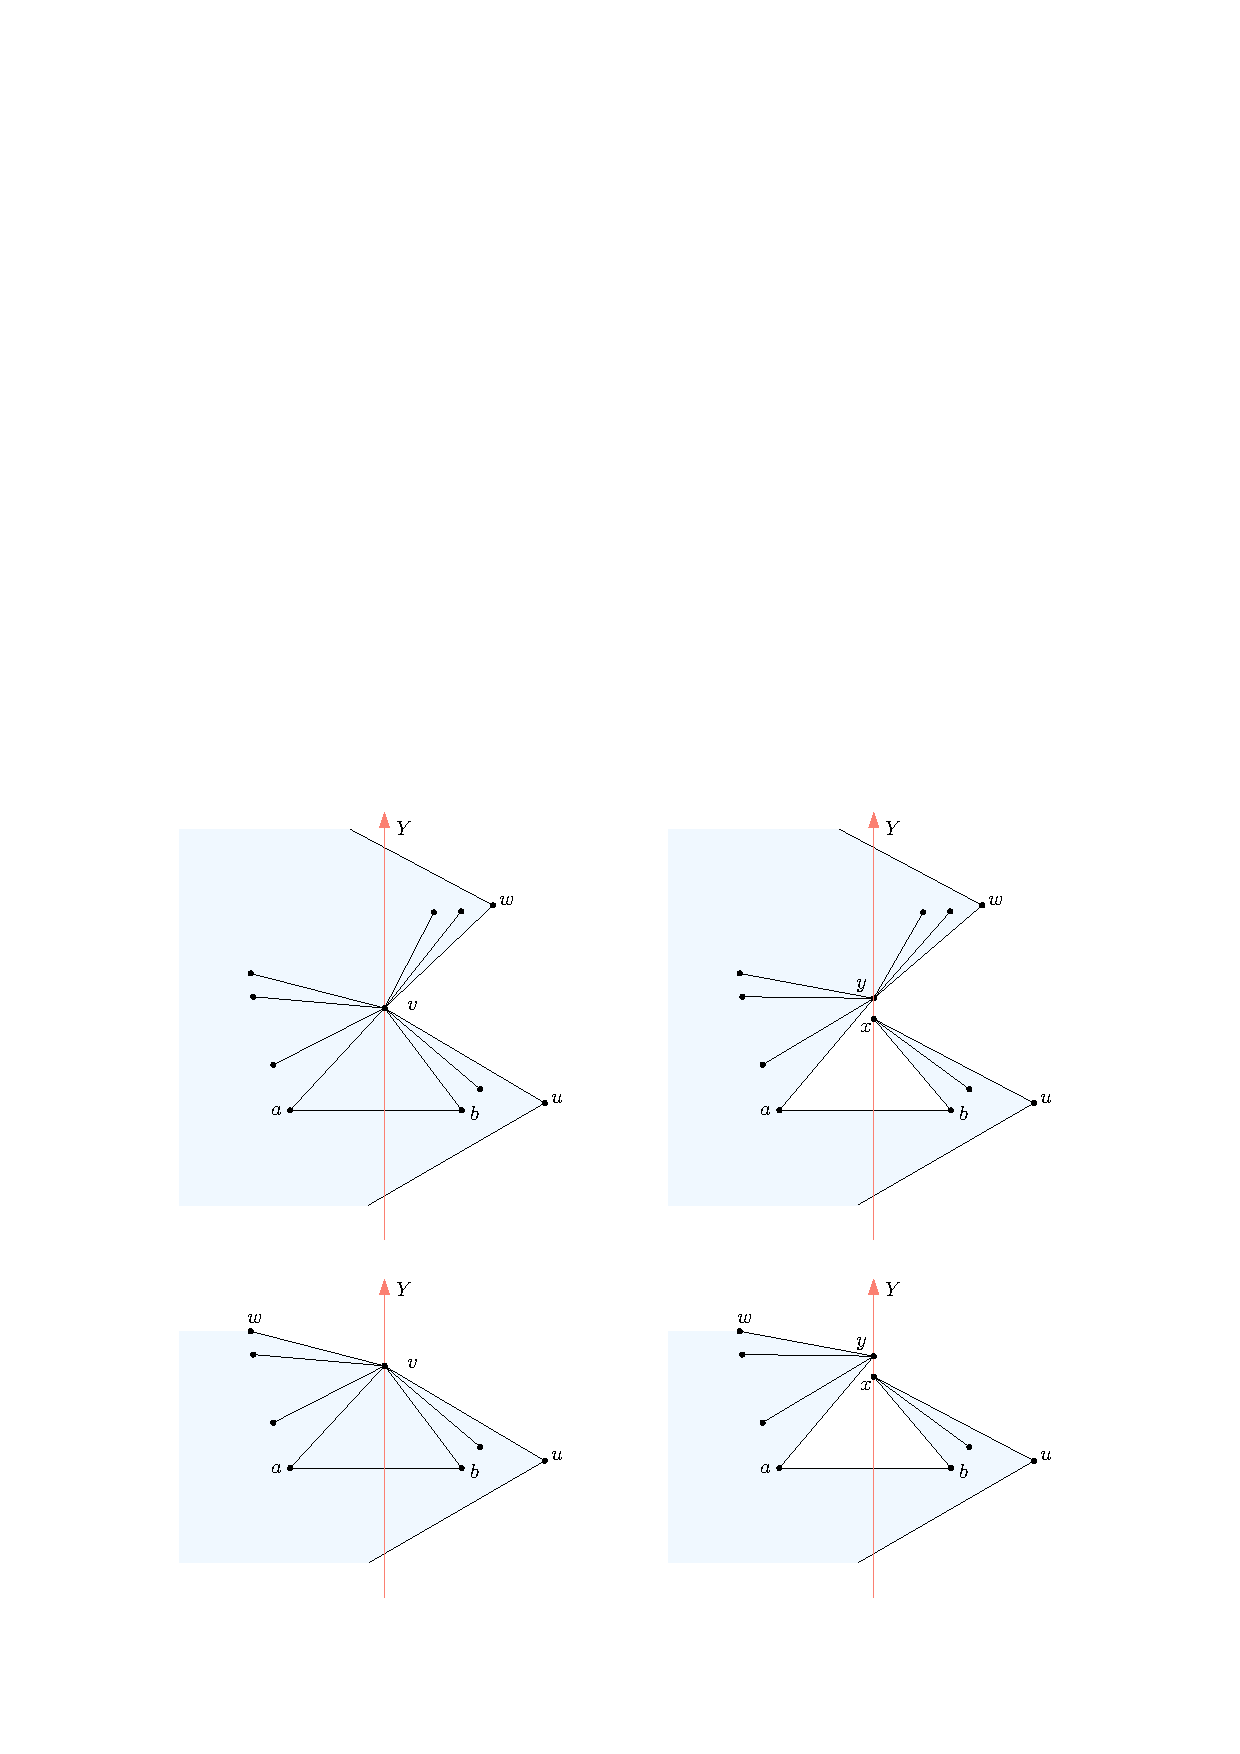
\includegraphics{figs/open-a-triangle}}
		\caption{Proof of \lemref{partition-extended} with a vertex
			$v$ on $Y$. Integrating a triangle in the outer face.}
		\figlabel{lemma-y-3}
	\end{figure}
	
	
	
	
	{\em Case 2}. The cycle $F$ contains no vertex on $Y$.
	Then $F$ contains at least four vertices. Since $Y$ intersects
	every edge of $F$, we have that $F$
	contains three consecutive vertices
	$u,v,w$ such that $Y$ exits an inner face through $uv$ and enters
	an inner face through $vw$, see \figref{lemma-y-4}.
	This implies that $v$ is a reflex vertex
	of some inner face $q=vabc$ of $G$.  Indeed, $vc$ is the first edge
	incident to $v$ crossed by $Y$ and $va$ is the last such edge.
	We construct a new graph $G'$ by splitting $v$ into two vertices $x$
	and $y$. We make the vertex $x$ adjacent to $u$ and every neighbor
	$z$ of $v$ such $Y$ intersects $vz$ before $vu$.  We make
	$y$ adjacent to all of $v$'s neighbors that are not adjacent to $x$.
	In $G'$, $q$ is part of the outer face, so $G'$ has one less inner
	face than $G$, hence induction applies.
	
	\begin{figure}
		\centering{\includegraphics{figs/lemma-y}}
		\caption{Proof of \lemref{partition-extended} for a reflex
			vertex $v$. Integrating a quadrilateral in the outer face.}
		\figlabel{lemma-y-4}
	\end{figure}
	
	
	
	This finishes the description of how we modify $G$ into $G'$. Every edge of $G'$ inherits its classification as an $H$-edge from its corresponding edge in $G$. We have to show that $G'$ satisfies Properties~(PR1)--(PR4). Actually Property~(PR1) is the only property that needs to be discussed, as the other properties follow trivially from the fact that $G$ satisfies them. 
%	Indeed,  $G'$ some of the $\prec$-relations involving edges incident to $v$ are missing, but no new ones are introduced, so $G'$ still
%	satisfies Condition~4.
%	The same argument applies to
%	Conditions~2 and~3. Some adjacent edges in $G$ might no longer be adjacent
%	in $G'$, but this makes Condition 2 and 3 only weaker.
%	
%	
	
	First, note that all the edges incident to the new vertices $x$ or $y$ were incident to $v$
	before, and thus they are $H$-edges. Second, all the edges incident to any boundary vertex of $G'$ that is also a boundary vertex of $G$ are $H$-edges, since the edges of $G'$ inherit their classification as $H$-edges from their corresponding edges in $G$. It remains to deal with the boundary vertices of $G'$ that are inner vertices of $G$.  
	
	In Case 1 we have two boundary vertices of $G'$, namely $a$ and $b$, which are inner vertices of $G$. Note that $a$ and $b$ do not lie on~$Y$. By Property~(PR1) for $G$, we have that $va$ and $vb$ are $H$-edges, since they are incident to the boundary vertex $v$. From the ordering constraints around $a$ and $b$ we get $va\prec ab\prec vb$
	or
	$vb\prec ab\prec va$, and thus, by Property~(PR4) for $G$, we have $ab\in H$.
	Now we have two $H$-edges $va$ and $ab$ incident to $a$,
	and by Property~(PR2) for $G$ all the edges incident
	to $a$ belong to $H$. It follows that all the edges incident to $a$ in $G'$ are $H$-edges, and similarly for~$b$.
	
	In Case~2 we have three boundary vertices of $G'$, namely $a$, $b$, and $c$, which are inner vertices of $G$. By Property~(PR1) for $G$, we have that $va$ and $vc$ are $H$-edges, since they are incident to the boundary vertex $v$. Consider the quadrilateral $q=vabc$ of $G$. By the ordering constraints, we get
	$vc \prec bc\prec ba\prec va$ or $va \prec ba\prec bc\prec vc$,
	depending on whether $v\in L$ or $v\in R$, respectively. Thus, by Property~(PR4) for $G$, the edges $bc$ and $ba$ are also $H$-edges. The vertex $b$ does not lie on $Y$. The vertex $a$ might lie on $Y$ or not, but if it does, then the two incident edges $va$ and $ab$ lie in the same half-plane.
	The same holds for $c$. Thus by Properties~(PR2) or~(PR3) for $G$ all the edges incident
	to $a$, $b$ and $c$ in $G$ belong to $H$. It follows that all the edges incident to $a$, $b$, and $c$ in $G'$ are $H$-edges.
	
	
	
	%   By Conditions~1 and 2, all edges incident to $v$ are $H$-edges and $v$
	%   is a reflex vertex of $q$. Therefore all edges of $q$ are $H$-edges.
	Since $G'$ satisfies Properties~(PR1)--(PR4) induction applies and all the edges of $G'$ (and thus all the edges of $G$) are $H$-edges. This completes the proof.
\end{proof}
